\chapter{Préliminaires}
\label{cp:preliminaires}

Avant de commencer à détailler la stratégie utilisée, il est nécessaire de présenter certaines notions sur lesquelles elle repose.

\section{Tas-Min}
\label{sec:tas-min}

Un Tas-min est une structure de données qui permet de stocker un ensemble d'éléments et de les récupérer dans un ordre particulier. 
C'est un cas particulier d'une file de priorité, où l'élément ayant la plus petite priorité est toujours en tête de file.
\newline\newline
Notre Tas-min est implémenté sous forme d'un tableau d'entiers, où chaque élément est un nœud de l'arbre binaire représentant le tas.
Les indices des éléments sont choisis de manière à ce que le fils gauche de l'élément à l'indice $i$ soit à l'indice $2i + 1$ et le fils droit à l'indice $2i + 2$.
La racine de l'arbre est à l'indice 0.

\begin{figure}[!htpb]
    \centering
    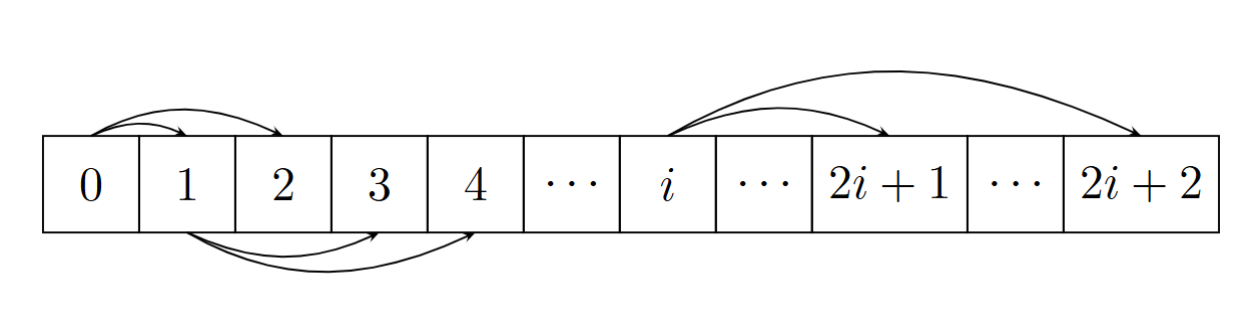
\includegraphics[width=0.9\linewidth]{Figures/array.png}
    \caption[Représentation d'un Tas-min sous forme de tableau.]{Représentation d'un Tas-min sous forme de tableau.}
    \label{fig:array}
\end{figure}

Pour gérer les Tas-min, nous avons besoin de trois procédures : \texttt{insert}, \texttt{modify\_}
\newline
\texttt{priority} et \texttt{extract\_min}.
La première permet d'ajouter un élément au tas, la deuxième de modifier la priorité d'un élément et la troisième de récupérer l'élément de priorité minimale.
\newline
On sait que l'élément de priorité minimale est toujours à la racine de l'arbre, on peut donc le récupérer en temps constant.
En cas d'insertion, de suppression ou de modification de priorité, on doit s'assurer que le tas reste bien un Tas-min.
Pour cela, on utilise une des deux procédures suivantes : \texttt{percolate\_up} et \texttt{percolate\_down}.

\subsection{Procédure \texttt{insert}}

On ajoute l'élément à la fin du tableau et on appelle \texttt{percolate\_up} pour s'assurer que le tas reste un Tas-min.
La procédure \texttt{percolate\_up} remonte l'élément ajouté tant que son parent a une priorité plus grande que la sienne.
\newline\newline
Son pseudo code est le suivant :

\begin{listing}[!htpb]
    \begin{minted}{text}
    Procédure percolate_up
    Parametres :
        @heap en tas-min
        i en entier
    Debut
        Tant que heap.priority[i] < heap.priority[(i - 1) / 2] et i > 0
            Echanger(heap.array, i, (i - 1) / 2)
            Echanger(heap->priority, i, (i - 1) / 2)
            i <- (i - 1) / 2
        Fin Tant que
    Fin
    \end{minted}
    \caption{Procédure \texttt{percolate\_up}.}
    \label{listing:percolate_up}
\end{listing}

\subsection{Procédure \texttt{modify\_priority}}

On modifie la priorité de l'élément et on appelle \texttt{percolate\_up} pour s'assurer que le tas reste un Tas-min.

\newpage

\subsection{Procédure \texttt{extract\_min}}

On récupère l'élément de priorité minimale, on le remplace par le dernier élément du tableau et on appelle \texttt{percolate\_down}.
La procédure \texttt{percolate\_down} descend l'élément remplacé jusqu'à ce que ses fils aient une priorité plus grande que la sienne.
\newline\newline
Son pseudo code est le suivant :

\begin{listing}[!htpb]
    \begin{minted}{text}
    Procédure percolate_down
    Parametres :
        @heap en tas-min
        i en entier
    Declarations :
        current, left, right en entier
    Debut
        current <- i
        left <- 2 * i + 1
        right <- 2 * i + 2

        Si left < heap.size et heap.priority[left] < heap.priority[current]
            current <- left
        
        Si right < heap.size et heap.priority[right] < heap.priority[current]
            current <- right
        
        Si current != i
            Echanger(heap.array, i, current)
            Echanger(heap.priority, i, current)
            percolate_down(heap, current)
    Fin
    \end{minted}
    \caption{Procédure \texttt{percolate\_down}.}
    \label{listing:percolate_down}
\end{listing}

\subsection{En C}

En C, on utilise une structure \texttt{min\_heap} pour représenter le Tas-min.

\begin{listing}[!htpb]
    \begin{minted}{c}
        typedef struct min_heap{
            int size; // Nombre d'éléments dans le tas
            int capacity; // Taille max du tas
            int* array; // Tableau des éléments
            float* priority; // Priorité des éléments
          } min_heap;
    \end{minted}
    \caption{Structure \texttt{min\_heap} en C.}
    \label{listing:c-min_heap}
\end{listing}

\newpage

On dispose en plus des fonctions suivantes pour manipuler les Tas-min :

\begin{listing}[!htpb]
    \begin{minted}{c}
        min_heap* create_min_heap(int);
        void free_min_heap(min_heap*);
        void percolate_up(min_heap*, int);
        void percolate_down(min_heap*, int);
        void insert(min_heap*, int, float);
        void modify_priority(min_heap*, int, float);
        int extract_min(min_heap*);
        bool is_member(min_heap*, int); 
    \end{minted}
    \caption{Fonctions sur les Tas-min en C.}
    \label{listing:c-min_heap-fonctions}
\end{listing}

\section{Algorithme A*}
\label{sec:a-star}

L'algorithme A* est un algorithme de recherche de chemin dans un graphe pondéré.
Il est basé sur l'algorithme de Dijkstra, mais utilise une heuristique pour guider la recherche.
L'algorithme A* est utilisé pour trouver le chemin le plus court entre un nœud de départ et un nœud d'arrivée dans un graphe.
\newline
Il utilise une file de priorité pour stocker les nœuds à explorer, dans laquelle la priorité d'un nœud est la somme du coût du chemin parcouru pour atteindre ce nœud et de l'estimation du coût restant pour atteindre le nœud d'arrivée (l'heuristique). 
On utilisera ici un Tas-min (\autoref{sec:tas-min}) pour implémenter cette file de priorité.

\subsection{Pseudo code}

\begin{longlisting}
    \begin{minted}{text}
        Fonction a_star en @path
        Parametres :
            origin en entier
            destination en entier
            level en niveau
        Déclarations :
            pat en @path
            u, v en entier
            h_v en flottant
        Début
            pat <- create_path // On initialise le chemin
            // pat.d est le tableau des distances, pat.p est le tableau des parents
            pat.d[origin] <- origin
            insert(pat.heap, origin, 0) // On ajoute le point d'origine a la file

            Tant que pat.heap n'est pas vide
                // Sommet courant, celui avec la priorite minimale
                u <- extract_min(pat.heap)

                Si u = destination
                    // On a trouve le bonus, on pourra remonter le chemin grace a pat.p
                    pat.found <- VRAI
                    Sortir de la boucle
                Fin Si

                Pour chaque action possible
                    Si l'action est valide // Dépend de level
                        v <- position apres l'action
                        h_v <- distance entre v et le bonus (l'heuristique)
                        Si pat.d[u] + poids de l'action < pat.d[v]
                            // Si on a trouve un chemin plus court
                            pat.d[v] <- pat.d[u] + poids de l'action
                            pat.p[v] <- u
                            Si v n'est pas dans la file
                                insert(pat.heap, v, pat.d[v] + h_v) // On l'ajoute
                            Sinon
                                // On modifie sa priorite
                                modify_priority(pat.heap, v, pat.d[v] + h_v)
                            Fin Si
                        Fin Si
                    Fin Si
                Fin Pour
            Fin Tant que

            Retourner pat
        Fin
    \end{minted}
    \caption{Fonction \texttt{a\_star}.}
    \label{listing:c-a_star}
\end{longlisting}

\subsection{En C}

En C, la fonction renvoie un chemin, qui est une structure contenant les informations nécessaires pour retrouver le chemin trouvé.
\newline\newline
On conserve le tableau des distances \texttt{d}, le tableau des parents \texttt{p}, un booléen \texttt{found} indiquant si le chemin a été trouvé et le Tas-min \texttt{heap}.
On garde le Tas-min pour les cas où il n'est pas vide (on n'a pas trouvé de chemin) et pour libérer la mémoire.

\begin{listing}[!htpb]
    \begin{minted}{c}
        typedef struct path{
            min_heap* heap; // File de priorité
            int* p; // Tableau des parents
            int* d; // Tableau des distances
            bool found; // Chemin trouvé ou non
            } path;
    \end{minted}
    \caption{Structure \texttt{path} en C.}
    \label{listing:c-path}
\end{listing}